% \documentclass[usenatbib,onecolumn]{mn2e}
\documentclass[usenatbib]{mn2e}

\usepackage{amsmath}
\usepackage{xspace}     % fixes spaces after custom commands
\usepackage{float}      % exact placement of figures (using \begin{figure}[H])
\usepackage[section,below]{placeins}   % gives a \FloatBarrier to force all floats to appear
\usepackage{subfigure}  % does what it says

\usepackage{graphicx}
% prefere pdf over png (better quality, lossless compression)
\DeclareGraphicsExtensions{%
  .pdf,.PDF,%
  .png,.PNG,%
  .jpg,.mps,.jpeg,.jbig2,.jb2,.JPG,.JPEG,.JBIG2,.JB2}

\newcommand{\apj}{ApJ}
\newcommand{\apjs}{ApJS}
\newcommand{\apjl}{ApJL}
\newcommand{\aap}{A{\&}A}
\newcommand{\aaps}{A{\&}AS}
\newcommand{\mnras}{MNRAS}
\newcommand{\aj}{AJ}
\newcommand{\araa}{ARAA}
\newcommand{\pasp}{PASP}
\newcommand{\pasj}{PASJ}
\newcommand{\nat}{Nature}
\newcommand{\nar}{New Astr Rev}

\def\half{{\textstyle\frac12}}
% makes it easier to have consistent writing, and easy change if needed
\newcommand{\spl}{SpaghettiLens\xspace}
\newcommand{\sw}{Spacewarps\xspace}

% shortcut for einstein radius (Text Greek Full Math)
\newcommand{\ER}{Einstein radius\xspace} % text
\newcommand{\ERg}[1][]{$\Theta_{\text{E#1}}$\xspace} % er in textmode with greek
\newcommand{\ERf}[1][]{Einstein radius $\Theta_\text{E#1}$\xspace} % full output
\newcommand{\ERm}[1][]{\Theta_\text{E#1}} % mathmode with greek symbol

%shortcuts for kappa
\newcommand{\kenc}[1][r]{$\kappa_\text{encl}(#1)$\xspace}
\newcommand{\kap}[1][r]{$\kappa(#1)$\xspace}

% shorcuts for refs (use capital for beginning of sentence)
% first 3 are for the real layz people..
\newcommand{\fref}[1]{\ref{fig:#1}}
\newcommand{\sref}[1]{\ref{sec:#1}}
\newcommand{\tref}[1]{\ref{tab:#1}}
\newcommand{\figref}[1]{Figure~\ref{fig:#1}}
\newcommand{\secref}[1]{Section~\ref{sec:#1}}
\newcommand{\tabref}[1]{Table~\ref{tab:#1}}
\newcommand{\Figref}[1]{Figure~\ref{fig:#1}}
\newcommand{\Secref}[1]{Section~\ref{sec:#1}}
\newcommand{\Tabref}[1]{Table~\ref{tab:#1}}

% shortcut for ASW000xxxx
\newcommand{\asw}[1]{ASW000#1\xspace}
\newcommand{\model}[2][Model~]{#1#2\xspace}

%degrees
\newcommand{\dgr}{^{\circ}}

%more abbrevs
\newcommand{\tgeom}{t_{\rm geom}}
\newcommand{\tgrav}{t_{\rm grav}}
\newcommand{\subcirc}{{\lower.33ex\hbox{$\circ$}}}
\newcommand{\subbullet}{{\lower.33ex\hbox{$\bullet$}}}


% todo annotations on side in red. easy to search for at the end
% !!! REMOVE THIS LINES FOR FINAL COMPILE
%
\usepackage{setspace}    % remove this pgk for final compile!! 
\usepackage{color}    % well... color...

%\newcommand{\todo}[2][red]{%
%\textcolor{#1}{\textbullet}%
%\marginpar{\colorbox{#1}{\parbox{\marginparwidth}{%
%\setstretch{0.4}\sffamily\textcolor{black}{\scriptsize{#2}}}}}}

\newcommand{\needfig}[1][]{%
\colorbox{yellow}{\parbox{0.5\textwidth}{%
\vspace{0.5cm}\setstretch{0.5}\textcolor{black}{\scriptsize{fig #1}}\vspace{0.5cm}}}%
\marginpar{\colorbox{yellow}{\parbox{\marginparwidth}{%
\setstretch{0.4}\sffamily\textcolor{black}{\scriptsize{fig}}}}}}

\setlength{\marginparsep}{0mm}
\setlength{\marginparwidth}{2.2cm}

\newcommand{\needcite}[1][]{\todo[green]{cit #1}}
\newcommand{\needref}[1][]{\todo[cyan]{ref #1}}
\newcommand{\needchk}[1][]{\todo[red]{chk #1}}

% \\\ END OF REMOVAL SECION

\newlength{\myplotswidth}
\setlength{\myplotswidth}{0.4\linewidth}

\newcommand{\hr}{\vspace{5mm}\noindent\rule{0.8\textwidth}{0.4pt}\vspace{5mm}}


\begin{document}




\title{Lens Modeling in \sw}

\author[Kueng et al]{Rafael Kueng,$^{1}$
Phil Marshall,$^{2}$
Anupreeta More,$^{3}$
Aprajita Verma,$^{4}$
Amit Kapadia,$^{5}$
\newauthor
Elisabeth Baeten,$^{6}$
Claude Cornen,$^{6}$
Christine McMillan,$^{6}$
Julianne Wilcox,$^{6}$
\newauthor
Jonas Odermatt,$^{7}$
Jonathan Coles,$^{8}$
Surhud More$^{3}$
and Prasenjit Saha$^{1}$ \\
$^{1}$Physik-Institut, University of Zurich, 190 Winterthurerstrasse, 8057, Zurich, Switzerland\\
$^{2}$Kavli Institute for Particle Astrophysics and Cosmology, Stanford University, 452 Lomita Mall, Stanford, CA 94035, USA\\
$^{3}$Kavli Institute for the Physics and Mathematics of the Universe, University of Tokyo, 5-1-5 Kashiwanoha, Kashiwa-shi 277-8583, Japan\\
$^{4}$Oxford Astrophysics, Keble Road, Oxford OX1 3RH, UK\\
$^{5}$Adler Planetarium, 1300 S. Lake Shore Drive, Chicago, IL 60605, USA\\
$^{6}$Spacewarps\\
$^{7}$Kantonsschule Zug, L\"ussiweg 24, 6300 Zug, Switzerland\\
$^{8}$Exascale Computing Lab, Versailles Saint-Quentin-en-Yveline University, 55 Avenue des Etats Unis, 78000, Versailles, France}

\maketitle

\input partA

\input partB

\input partC

\bibliographystyle{mn2e}
\bibliography{bib/ms}

\end{document}



In \secref{Fermat}, for the sake of a more intuitive
explanation, we suppressed some constant factors in
equations \eqref{eq:Ageom}, \eqref{eq:Aarriv} and \eqref{eq:Poisson}.
Here we fill in the details.

First let us recall various distance formulas. Comoving distances
involve integrals of the type
\begin{equation}
\int \frac{dz}{\sqrt{\Omega_m(1+z)^3 + \Omega_\Lambda}}
%\raise.5ex\hbox{.}
\end{equation}
Specifically, the comoving distance $D_S$ from observer to source,
$D_{LS}$ from lens to source, and $D_L$ from observer to lens are
given by the above integral, with limits as follows.
\begin{equation}
\begin{aligned}
&D_S    &                                &\int_0^{z_S} \\
\noalign{\medskip}
&D_{LS} & = \frac c{H_0} \ \times \quad  &\int_{z_L}^{z_S} \\
\noalign{\medskip}
&D_L    &                                &\int_0^{z_L}
\end{aligned}
\end{equation}
Angular-diameter distances $d$ can be related to comoving distances
$D$ by scale factors, as follows.
\begin{equation}
\begin{aligned}
D_S &= (1+z_S) \, d_S \\
D_{LS} &= \frac{1+z_S}{1+z_L} \, d_{LS} \\
D_L &= (1+z_L) \, d_L
\end{aligned}
\end{equation}
Consequently, angular-diameter distances are always smaller than
comoving distances.  Moreover, while comoving distances can be simply
added, angular distances cannot:
\begin{equation}
d_S \neq d_L + d_{LS}
\end{equation}

Locations on the lens plane in angular coordinates on the sky, are
expressed as
\begin{equation}
(x,y) = d_L (\theta_x,\theta_y)
\end{equation}

The $A$ areas (with the implicit
constant factor that makes them time delays) and the $\kappa$ density are related to physical arrival
time $t$ and density $\Sigma$ as
\begin{equation}
\begin{aligned}
A           &= \frac{c}{(1+z_L)^2} \frac{D_L D_{LS}}{D_S} \times t \\
\kappa(x,y) &= \frac{4\pi G}{c^2} \frac{D_L D_{LS}}{D_S}
               \times \Sigma(x,y)
\end{aligned}
\end{equation}
Letting the source be offset at $(s_x,s_y)$ rather than at the
origin, we have
\begin{equation}
\begin{aligned}
t_{\rm geom} &= \frac{(1+z_L)^2}{2c} \frac{D_S}{D_L D_{LS}}
\left( (x-s_x)^2 + (y-s_y)^2 \right) \\
\nabla^2 t_{\rm grav} &= -(1+z_L)\frac{8\pi G}{c^3} \, \Sigma(x,y)
\end{aligned}
\end{equation}
We can now compare with equations (2.1) to (2.6)
from \cite{1986ApJ...310..568B}.
%% comparison to be explicited

\section{Miscellaneous}

Maybe discard \figref{ER_all_models}, since the essential information is there in \figref{ER_per_sim}.

\begin{figure}[htbp]
  \centering
    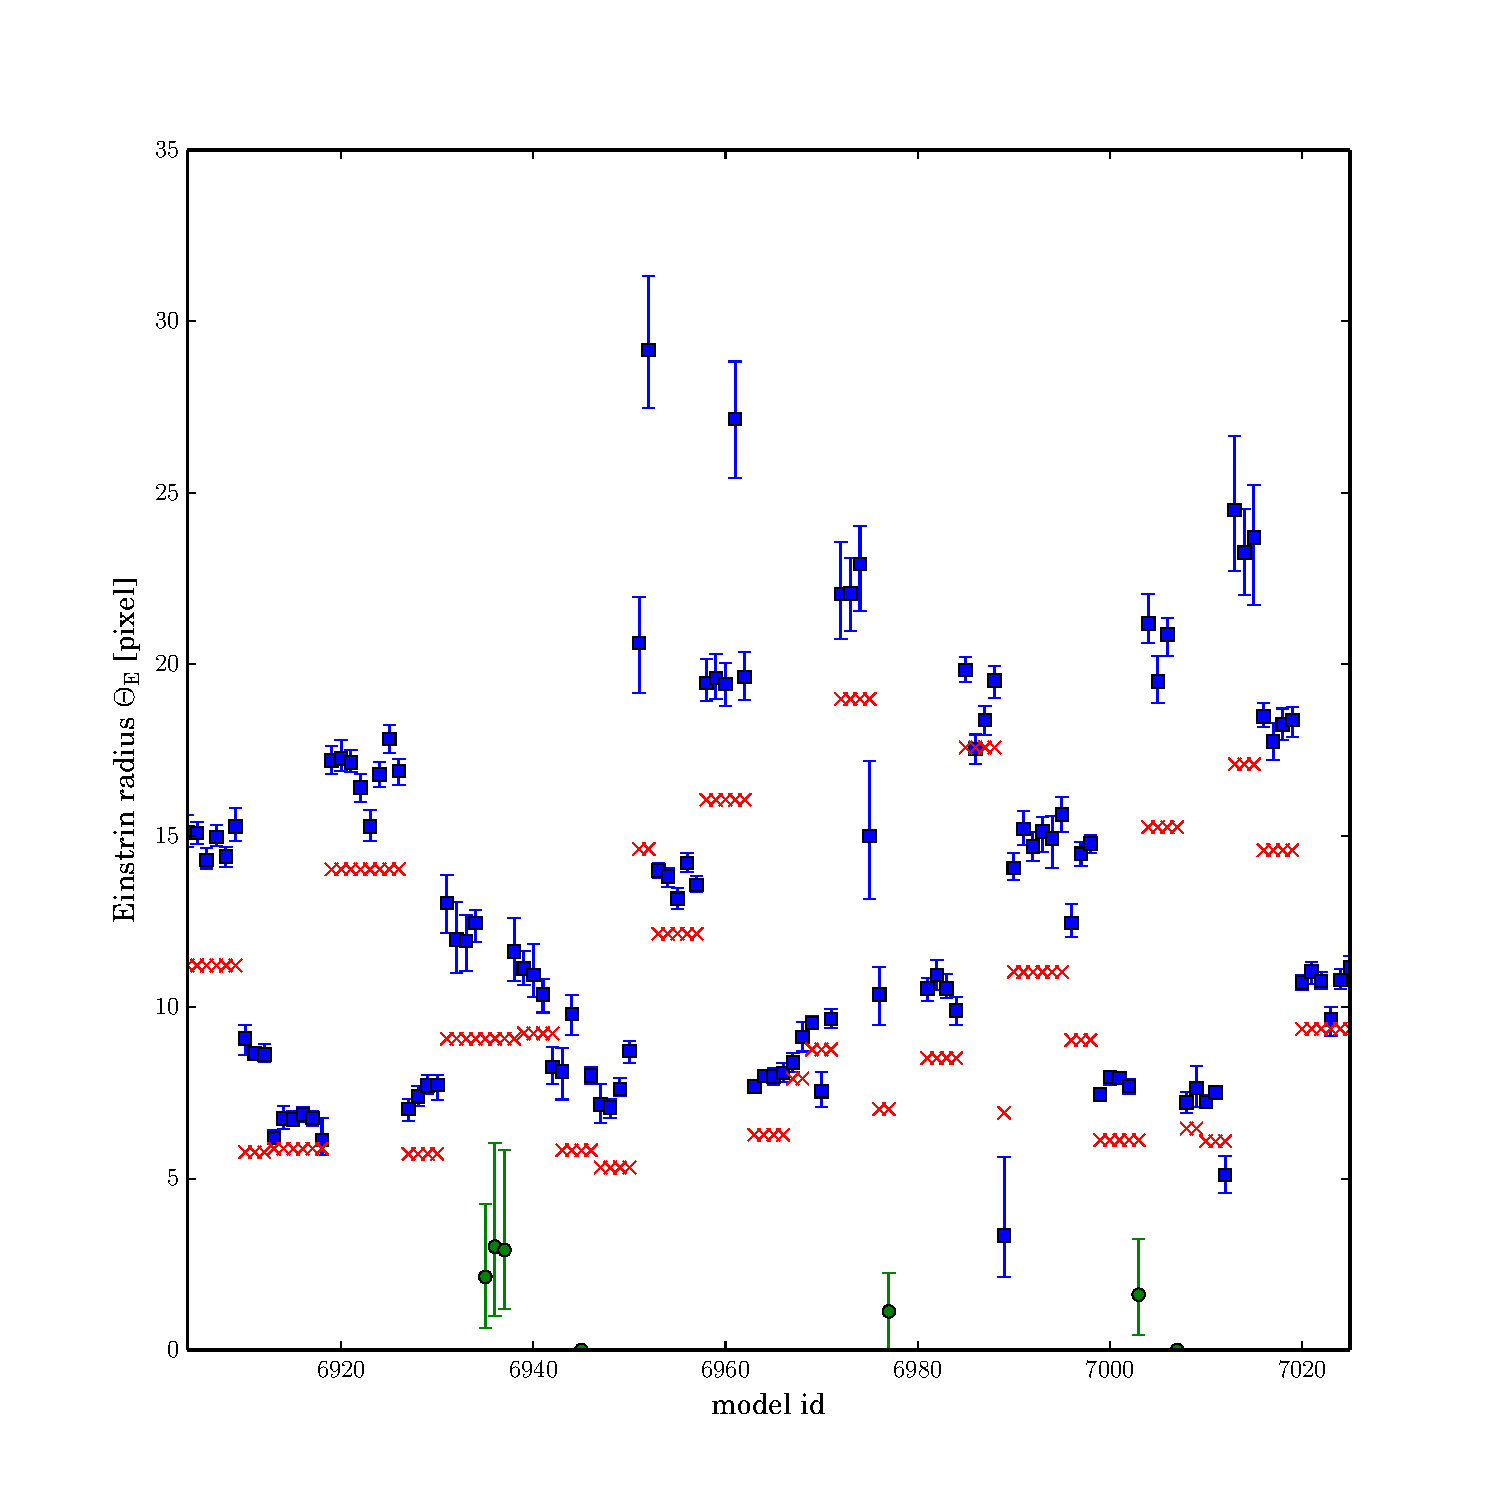
\includegraphics[width=0.90\linewidth]{fig/eR_1}
  \caption{\ERf for all models with estimated errors in blue squares, \ERg of simulation in red crosses}
  \label{fig:ER_all_models}
\end{figure}






